%\section{Methodology}\label{sec:methodology}
\colchunk[1]{%
        %EDUCATION\\*
        %\\*[.5\baselineskip]
        %\\*
%\titlespacing*{\subsection}{1pt}{1.1\baselineskip}{\baselineskip}        
\vspace{-40em}
\section{Select Distributed Algorithm}\label{subsec:algorithm}
The Minimum Dominating Set Approximation algorithm as presented by Alipour et al., is specified as:
%Within the graph algorithms, some SNN algorithms may be naturally more robust than others. For example, SNN algorithms that calculate the shortest path within graphs may automatically re-route if radiation imposed neuron-death occurs. However, since this research aims at determining the effectivity of brain adaptation mechanisms, a stricter test is found in algorithms that can fail to produce meaningful output if a single neuronal or synaptic property is changed. Therefore, 
%\begin{algorithm}%[h]%[1]
    %\caption{Distributed Algorithm for computing a total dominating set in a graph with given integer $m\geq 0$.}\label{alg:alipour}

%\KwData*
\textbf{Input:}\textit{Connected, planar, triangle-free graph of size $n$.}\\
%\KwResult*{\textit{Set of nodes that form a minimum total dominating set.}}
\textbf{Output:}\textit{Set of nodes that form a minimum total dominating set.}\\
%\setlist{nolistsep}
\vspace{-1.5em}
\begin{enumerate}[noitemsep]
\itemsep-1.5em
\item \textit{In the first round, each node $v_i$ chooses a random number $0<r_i<1$ and computes its weight $w_i=d_i+r_i$ and sends $w_i$ to its adjacent neighbours.}\\
\item \textit{In the second round, each node $v$ marks a neighbour vertex $v_i$ whose weight $w_i$ is maximum among all the other neighbours of $v$.}\\
\For{$m$ rounds}{
    \begin{enumerate}[noitemsep]
        \itemsep-1.5em
    \item \textit{Let $x_i$ be the number of times that a vertex is marked by its neighbour vertices, let $w_i=x_i+r_i$}\\
    \item \textit{Unmark the marked vertices.}\\
    \item \textit{Each vertex marks the vertex with maximum $w_i$ among its neighbour vertices.}\\
    \end{enumerate}
}
\vspace{1em}
\item \textit{The marked vertices are considered as the vertices in our total dominating set for $G$.}
\end{enumerate}
%\end{algorithm}

\section{Convert Algorithm to Spiking Neural Network(SNN)}\label{subsec:algo_to_snn}
%\vspace{-1.5em}
Next, an SNN implementation of this algorithm is generated using Leaky-Integrate-and-Fire (LIF) neurons. This implementation takes as input connected, triangle-free, planar graphs (E.g. Fig 1.). Then it converts these graphs into the specification of an SNN that is encoded in a new graph (E.g. Fig 2.). These graphs can then be simulated using the Lava backend by Loihi, or a custom networkx SSN simulator backend.

\section{Apply Adaptation Mechanism to SNN}\label{subsec:adaptation}
This default network is enhanced with strategically placed redundant neurons that are inhibited by the default network neurons. 


\section{Simulate Radiation on SNN}\label{subsec:}
Next, space radiation damage is simulated in the form of random neuron deaths. Redundant neurons can die too. \vspace{-7em}
\section{Compare SNN Performance With-/out Adaptation}\label{subsec:}
Algorithm performance is compared with/without the adaptation mechanism when exposed to radiation.\\
\\*[.5\baselineskip]
\\*
%\begin{figure}[]
%    \centering
%    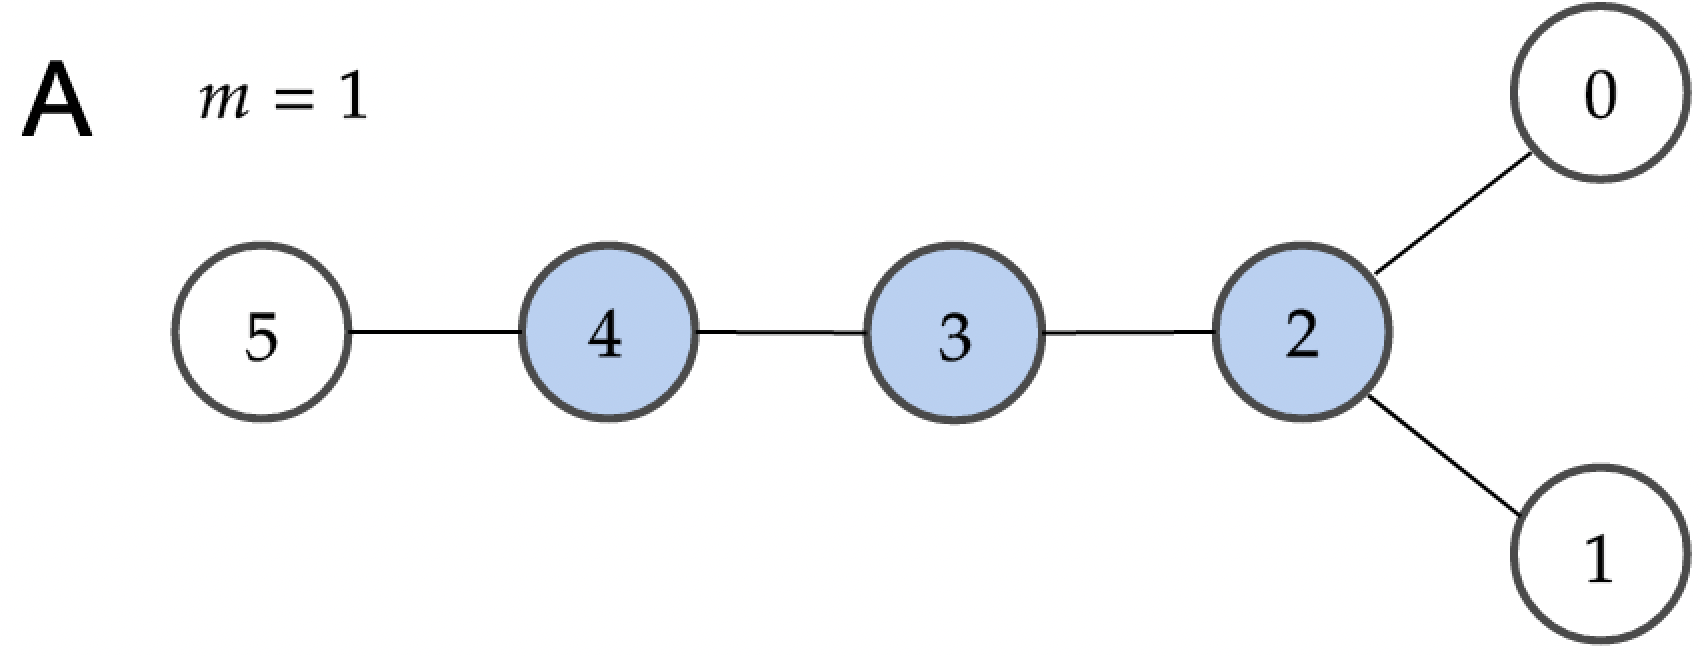
\includegraphics[width=8cm]{latex/Images/input_graph_G_6_0_alternative1.png}
%    \caption{Example input graph. For $m=1$ the algorithm still selects 3 nodes as it is an approximation of the MDS.}
%    \label{fig:input_graph}
%\end{figure}
%\hspace{-3em}
\vspace{-45em}
\begin{rudifig}{0.49\hsize}{Fig. 1: Input Graph}
%\begin{rudifig}{Fig. 1: Input Graph}
    \hspace{-1.5em}
    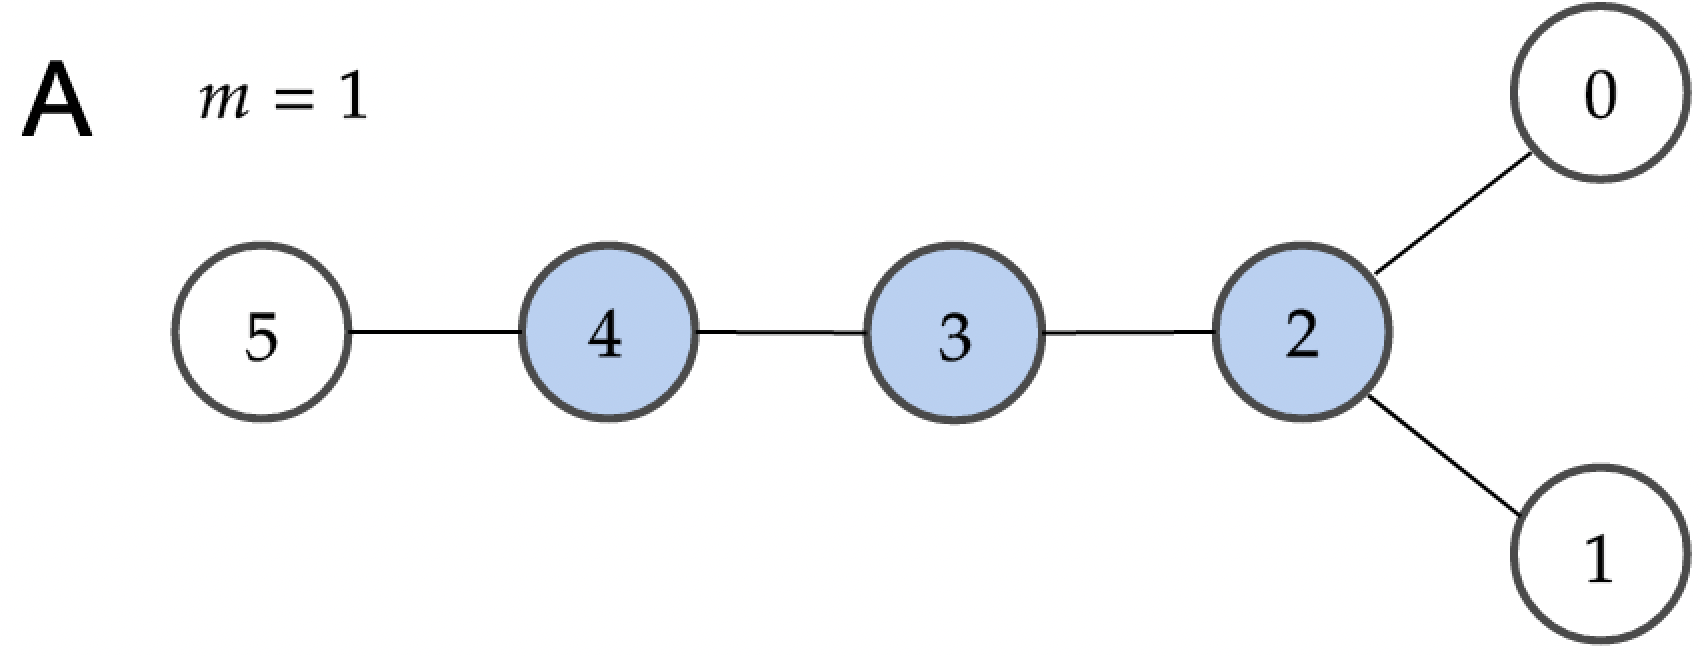
\includegraphics[width=1.1\linewidth]{latex/Images/input_graph_G_6_0_alternative1.png}
    %\caption{Example input graph. For $m=1$ the algorithm still selects 3 nodes as it is an approximation of the MDS.}
    \label{fig:input_graph}
\end{rudifig}
% Non poster image:
%\begin{figure}[H]
%    \centering
%    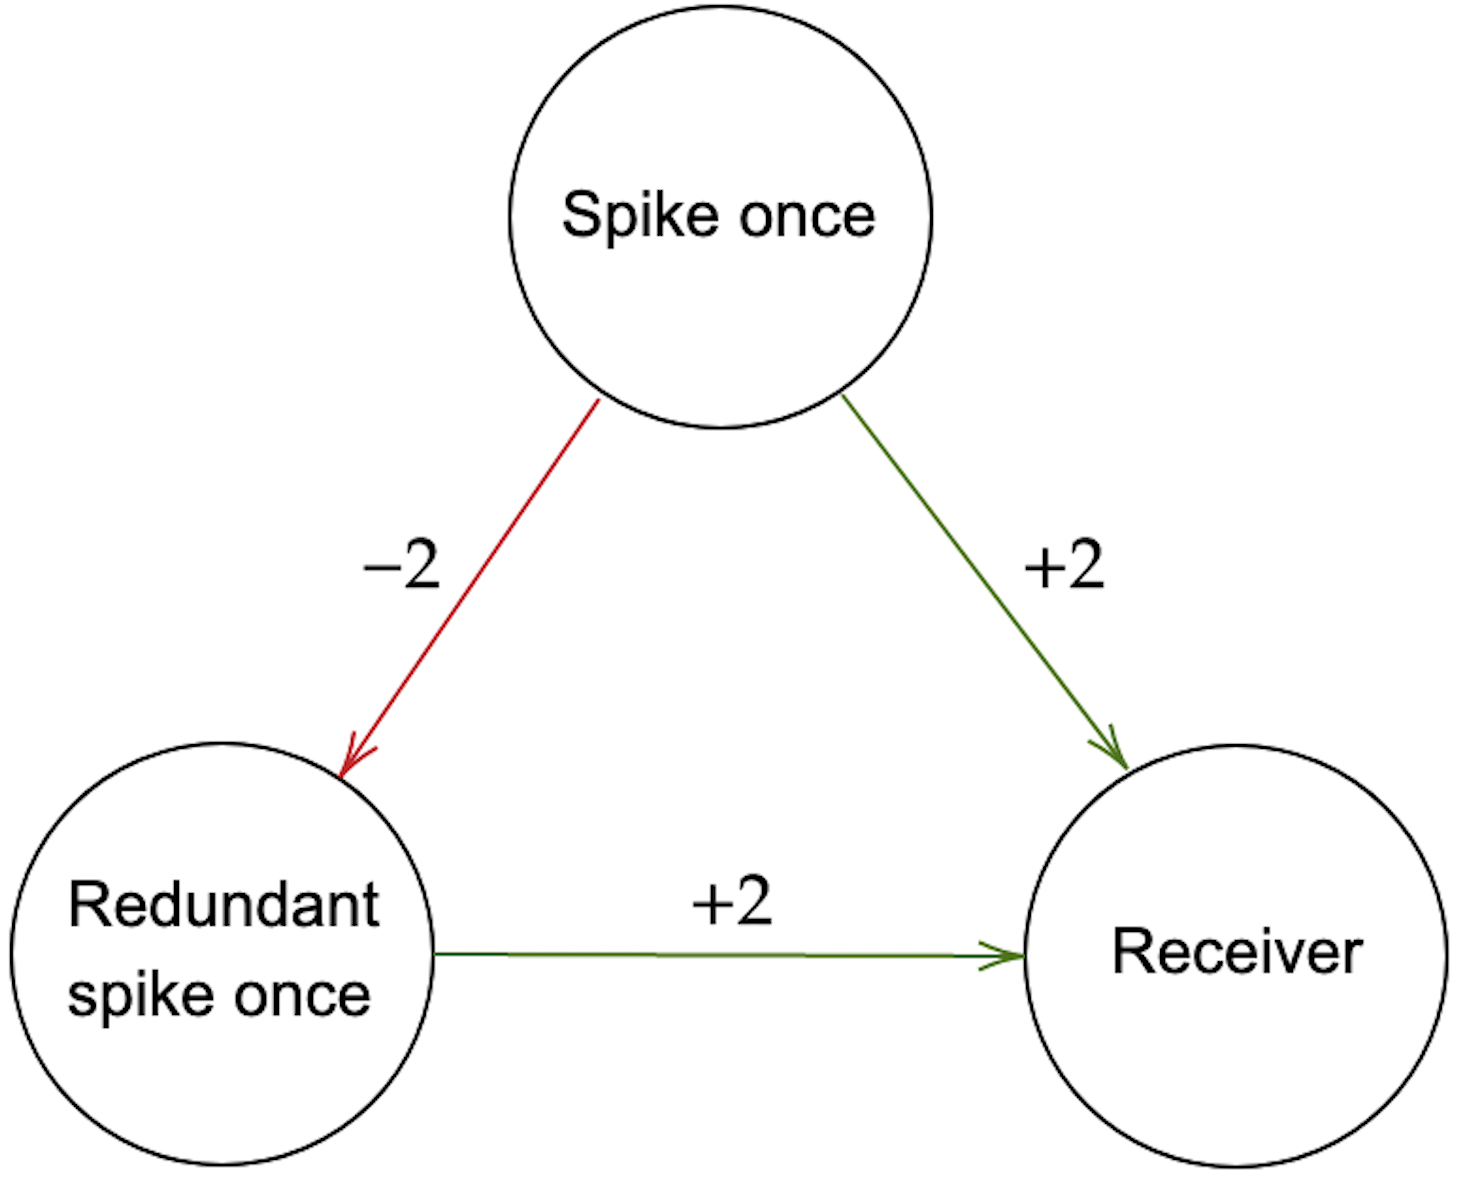
\includegraphics[width=.5\linewidth]{latex/Images/brain_adaptation_alternative.png}
%    \caption{Alternative neural pathway for a redundancy of the spike\_once neuron. If the spike\_once neuron dies due to simulated radiation-induced SEEs ($vth=inf$), the redundancy neuron inhibition is eliminated. Without inhibition, the redundant spike\_once neuron copies the spike\_once behaviour with a delay of 1 timestep.}
%    \label{fig:eg_brain_adaptation}
%\end{figure}
\begin{rudifig}{0.5\hsize}{Fig. 3: Redundancy}
    %\hspace{2em}
%\begin{rudifig}{Fig. 3: Redundancy}
    %
\includegraphics[width=\hsize]{ru_en_1}
    %\hspace{-1em}
    %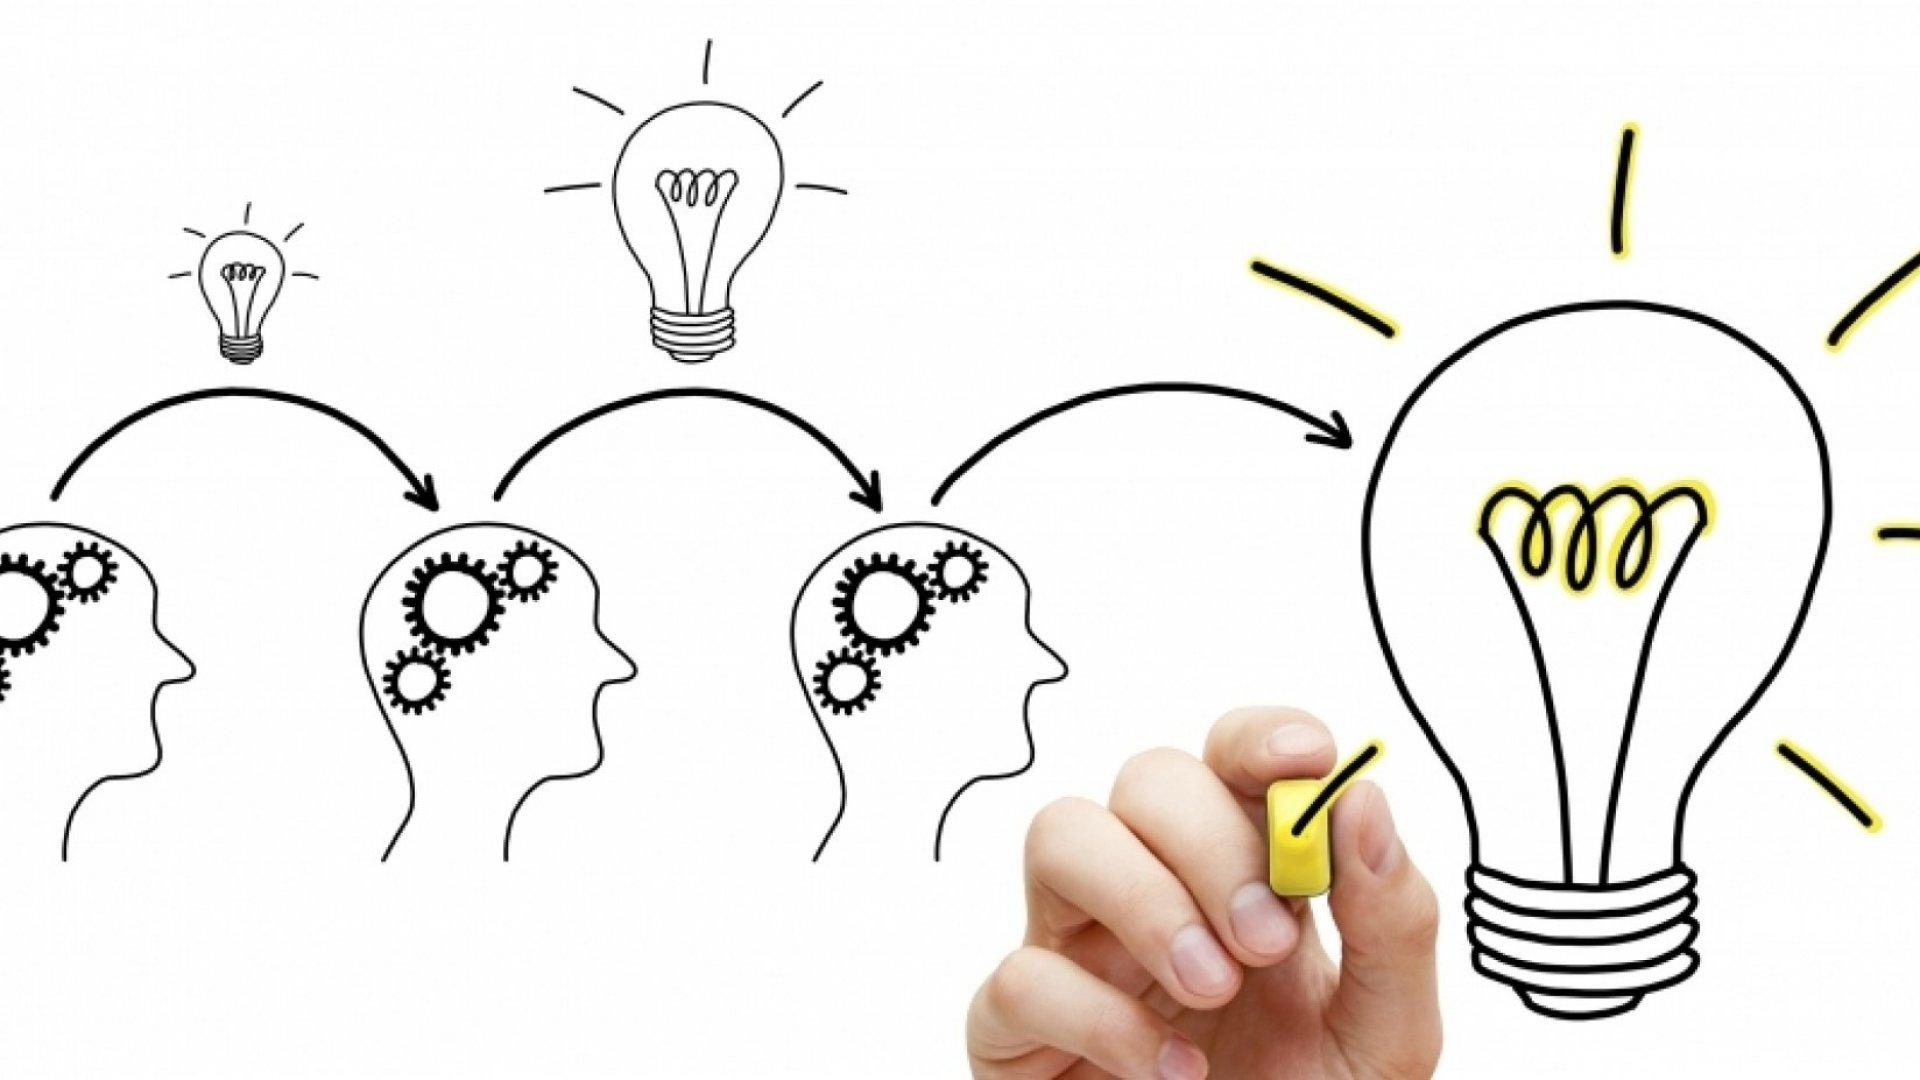
\includegraphics[width=700pt]{latex/Images/os0.jpg}
    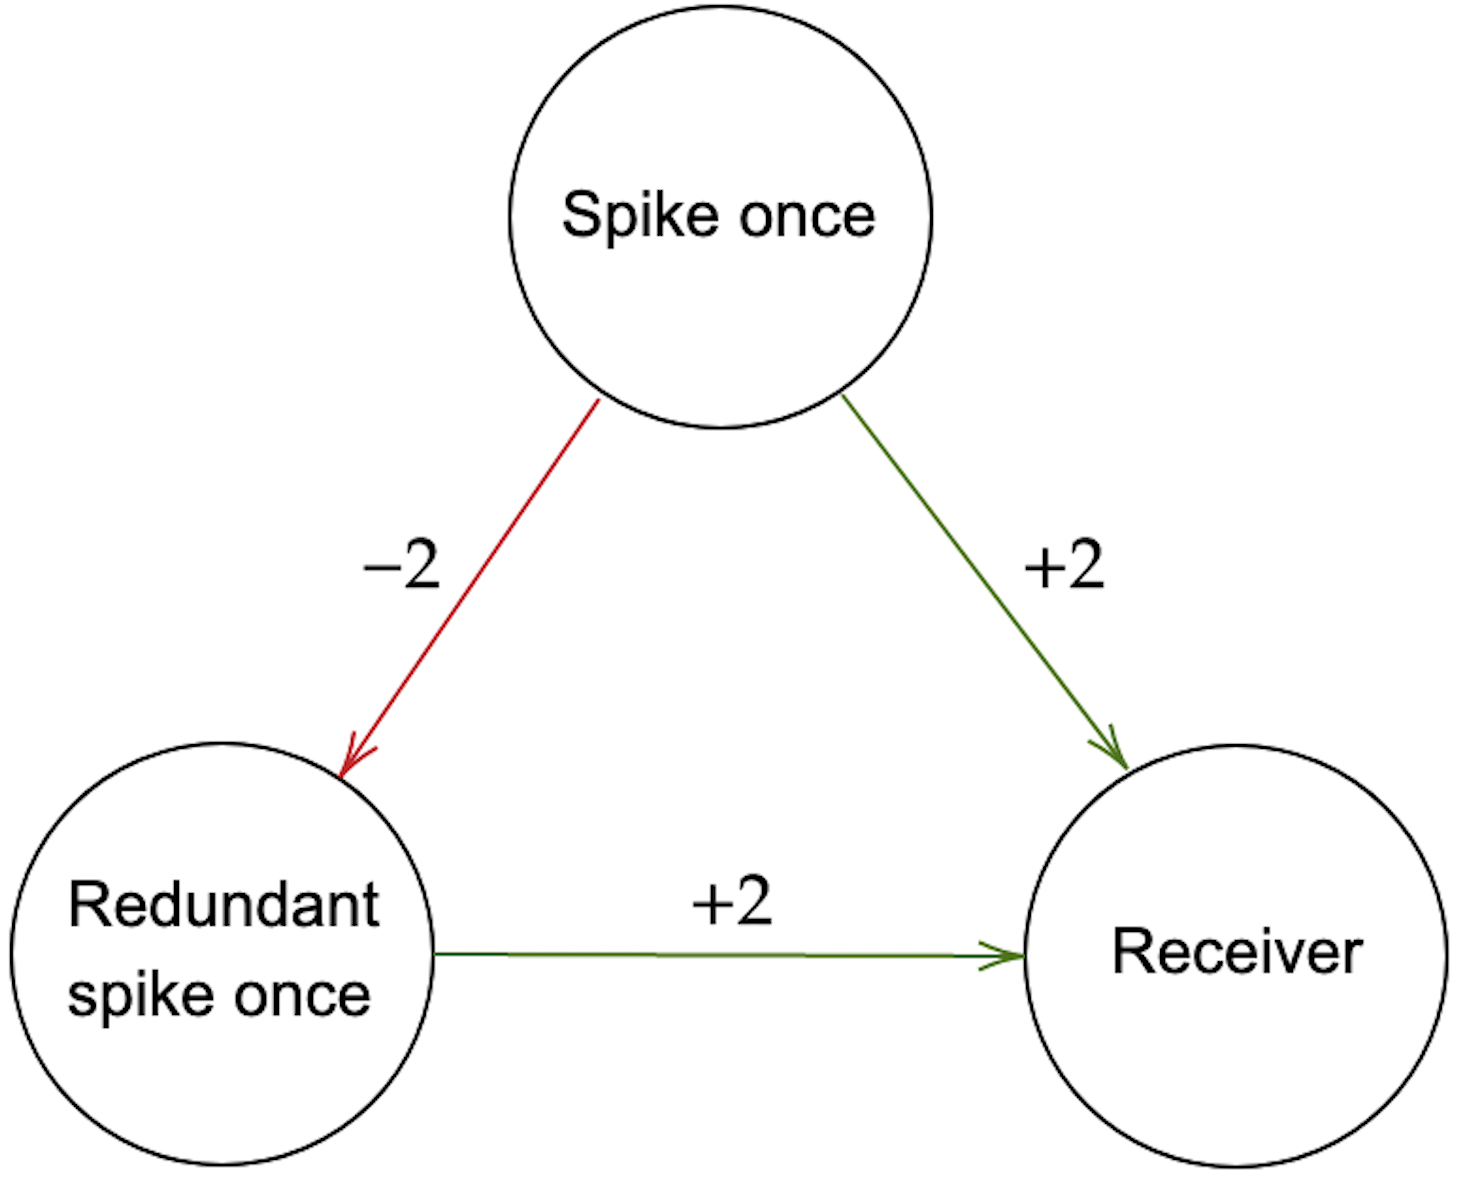
\includegraphics[width=1\linewidth]{latex/Images/brain_adaptation_alternative.png}
    %\caption{Alternative neural pathway for a redundancy of the spike\_once neuron. If the spike\_once neuron dies due to simulated radiation-induced SEEs ($vth=inf$), the redundancy neuron inhibition is eliminated. Without inhibition, the redundant spike\_once neuron copies the spike\_once behaviour with a delay of 1 timestep.}
    \label{fig:eg_brain_adaptation}
\end{rudifig}


\vspace{-15em}


}
\colchunk[2]{%
    \begin{rudifig}{1\hsize}{Fig. 2: Output SNN}
        %\vspace{-3em}
            %\hspace{-1em}
            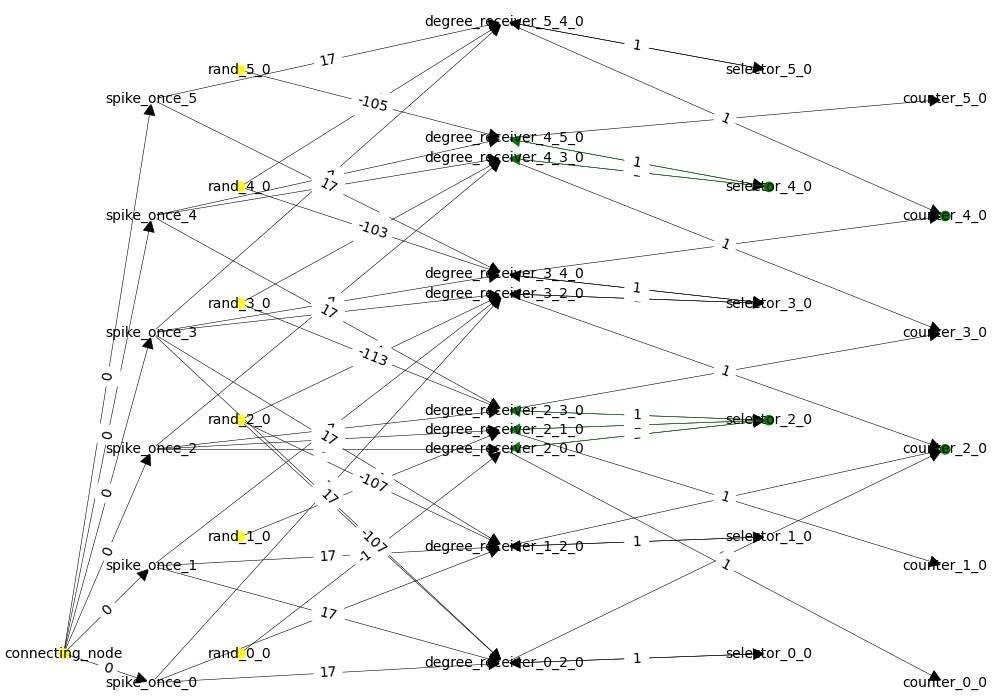
\includegraphics[width=1.\linewidth]{latex/Images/cropped.jpeg}
            %\caption{Example SNN encoding of algorithm to approximate MDS on the input graph of \cref{fig:input_graph}. This module is connected in series where the mark counter neuron takes up the role of spike\_once neuron in the next round of the approximation algorithm. For a more detailed description of the SNN implementation the reader is referred to Diehl et al. \cite{diehl}. %TODO: update to match updated input graph.
            %}
            \label{fig:encoded_snn}
        \end{rudifig}
        
        
        
\begin{rudifig}{1\hsize}{Fig. 4: Adaptation: Redundancy (And Radiation in Red)}
    %\hspace{-1.5em}
    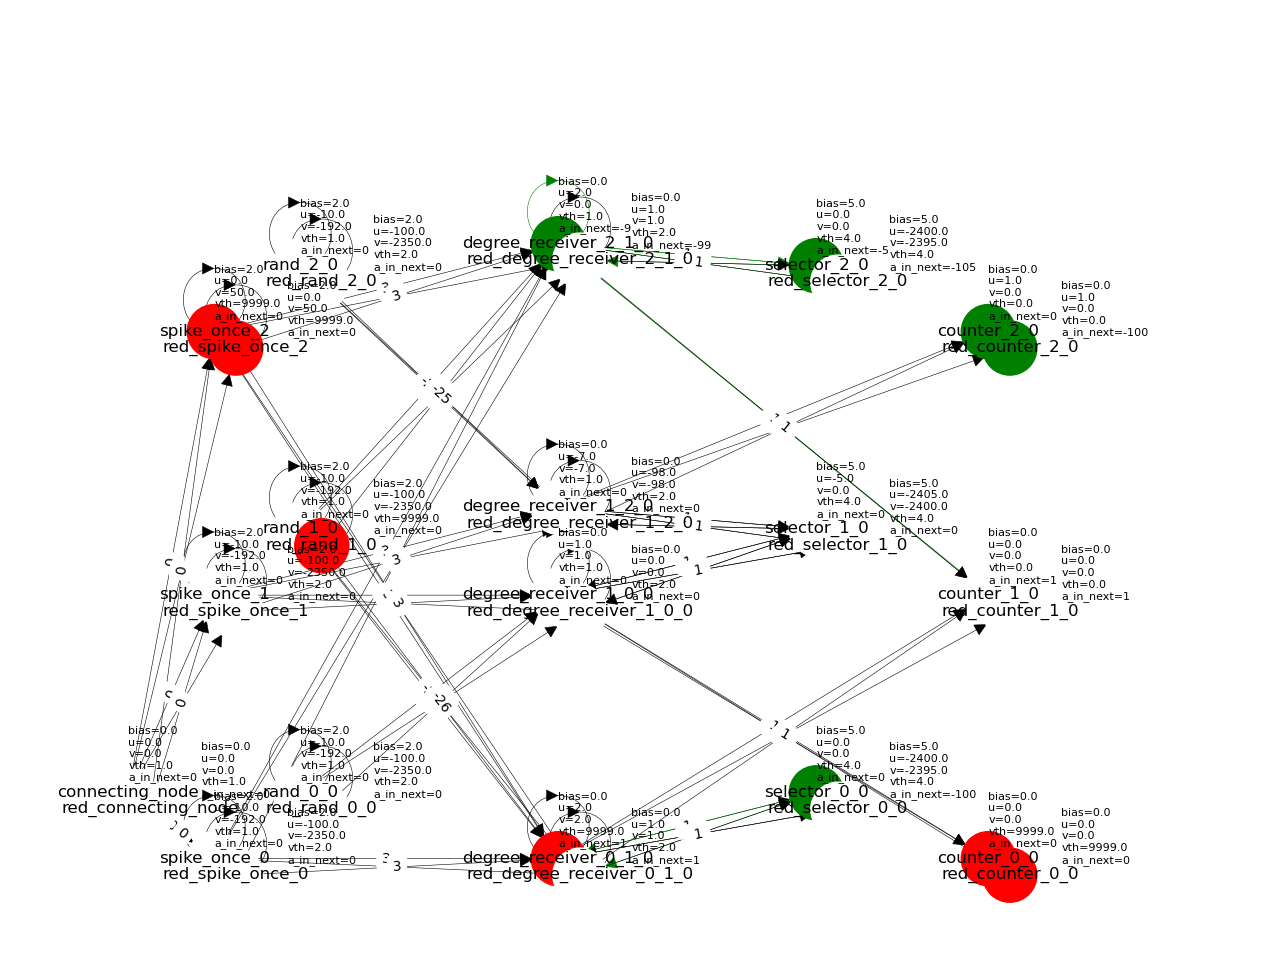
\includegraphics[width=1\linewidth]{latex/Images/rad_adapted.png}
    %\caption{Example SNN encoding of algorithm to approximate MDS on the input graph of \cref{fig:input_graph}. This module is connected in series where the mark counter neuron takes up the role of spike\_once neuron in the next round of the approximation algorithm. For a more detailed description of the SNN implementation the reader is referred to Diehl et al. \cite{diehl}. %TODO: update to match updated input graph.
    %}
    \label{fig:encoded_snn}
\end{rudifig}


}